\documentclass{article}
\usepackage[utf8]{inputenc}
\usepackage[icelandic]{babel}
\usepackage[T1]{fontenc}
\usepackage{graphicx}
\usepackage{mathtools}
\usepackage{amsmath}
\usepackage{amssymb}
\usepackage{minted}


\graphicspath{ {./} }
\title{Verkefni 4 - ghsr}
\author{ttb3@hi.is}
\date{\today}

\begin{document}
\maketitle


\section*{Verkefni 1}

\section*{Hvað gerði ég}
ég byrjaði á því að reikna binary margföldun tveggja og þriggja bita tölu þar sem báðar tölur voru eins stórar og þær gátu verið, þ.e. $111$ og $11$.
ég gerði þennan útreikning á blað og hreinskrifaði svo upp í excel og fékk þetta út:
\begin{center}
    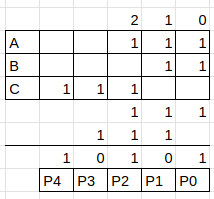
\includegraphics{imgs/Screenshot from 2022-03-11 10-17-35.png}
\end{center}

núna veit ég hvar carrybitar koma fram og get skrifað upp bitamargföldunartöflu, hvað heitir þessi týpa af töflum??, 
gerði það eins og með útreikningin, fyrst á blað svo í excel, svona endaði taflan:
\begin{center}
    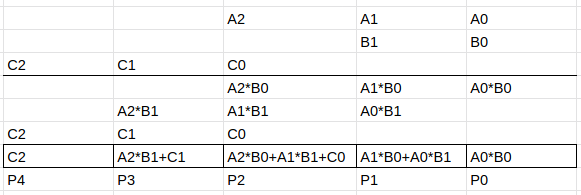
\includegraphics[scale=0.55]{imgs/Screenshot from 2022-03-11 10-23-10.png}
\end{center}

núna veit ég hvernig boolean jafna fyrir rás hvers og eins output lítur út og þá er voða lítið mál að teikna það upp í tölvunni:
\begin{center}
    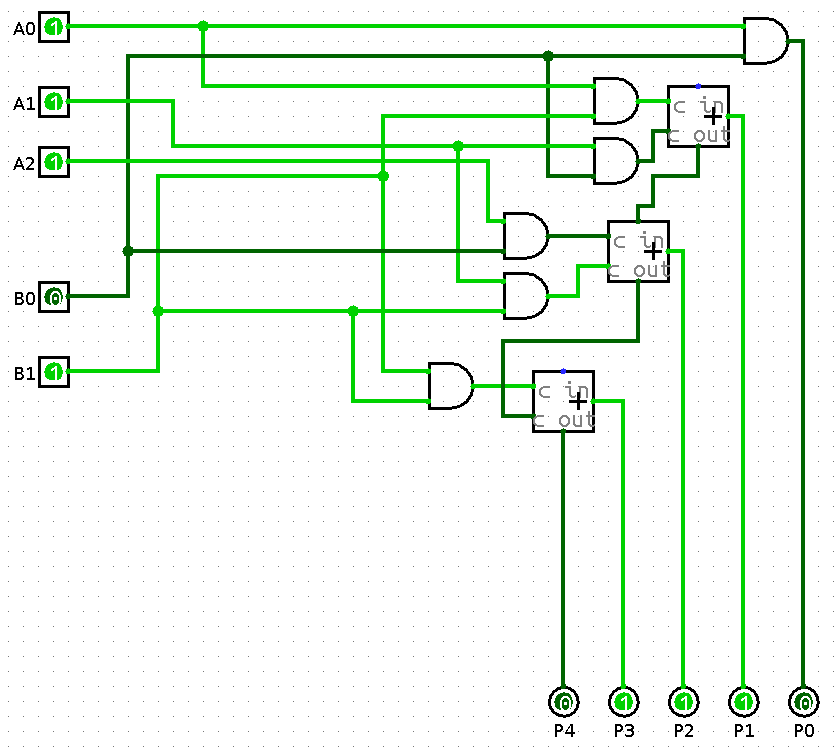
\includegraphics[scale=0.4]{imgs/Screenshot from 2022-03-11 10-51-59.png}
\end{center}

síðasta skrefið var svo bara að láta forritið herma rásina fyrir mig og athuga hvort hún sé rétt, sanntaflan lítur svona út:
\begin{center}
    \begin{tabular}{|c|c|c|c|c|c|c|c|c|c|}
    A0&A1&A2&B0&B1&P4&P3&P2&P1&P0\\
    hline
0&0&0&0&0&0&0&0&0&0\\
\hline
0&0&0&0&1&0&1&0&0&0\\
\hline
0&0&0&1&0&0&0&0&0&0\\
\hline
0&0&0&1&1&0&1&0&0&0\\
\hline
0&0&1&0&0&0&0&0&0&0\\
\hline
0&0&1&0&1&0&1&0&0&0\\
\hline
0&0&1&1&0&0&0&1&0&0\\
\hline
0&0&1&1&1&0&1&1&0&0\\
\hline
0&1&0&0&0&0&0&0&0&0\\
\hline
0&1&0&0&1&0&1&1&0&0\\
\hline
0&1&0&1&0&0&0&0&1&0\\
\hline
0&1&0&1&1&0&1&1&1&0\\
\hline
0&1&1&0&0&0&0&0&0&0\\
\hline
0&1&1&0&1&0&1&1&0&0\\
\hline
0&1&1&1&0&0&0&1&1&0\\
\hline
0&1&1&1&1&1&0&0&1&0\\
\hline
1&0&0&0&0&0&0&0&0&0\\
\hline
1&0&0&0&1&0&1&0&1&0\\
\hline
1&0&0&1&0&0&0&0&0&1\\
\hline
1&0&0&1&1&0&1&0&1&1\\
\hline
1&0&1&0&0&0&0&0&0&0\\
\hline
1&0&1&0&1&0&1&0&1&0\\
\hline
1&0&1&1&0&0&0&1&0&1\\
\hline
1&0&1&1&1&0&1&1&1&1\\
\hline
1&1&0&0&0&0&0&0&0&0\\
\hline
1&1&0&0&1&0&1&1&1&0\\
\hline
1&1&0&1&0&0&0&0&1&1\\
\hline
1&1&0&1&1&1&0&0&0&1\\
\hline
1&1&1&0&0&0&0&0&0&0\\
\hline
1&1&1&0&1&0&1&1&1&0\\
\hline
1&1&1&1&0&0&0&1&1&1\\
\hline
1&1&1&1&1&1&0&1&0&1\\
\hline
    \end{tabular}
\end{center}

\end{document}